% Options for packages loaded elsewhere
\PassOptionsToPackage{unicode}{hyperref}
\PassOptionsToPackage{hyphens}{url}
\PassOptionsToPackage{dvipsnames,svgnames,x11names}{xcolor}
%
\documentclass[
  letterpaper,
  DIV=11,
  numbers=noendperiod]{scrartcl}

\usepackage{amsmath,amssymb}
\usepackage{iftex}
\ifPDFTeX
  \usepackage[T1]{fontenc}
  \usepackage[utf8]{inputenc}
  \usepackage{textcomp} % provide euro and other symbols
\else % if luatex or xetex
  \usepackage{unicode-math}
  \defaultfontfeatures{Scale=MatchLowercase}
  \defaultfontfeatures[\rmfamily]{Ligatures=TeX,Scale=1}
\fi
\usepackage{lmodern}
\ifPDFTeX\else  
    % xetex/luatex font selection
\fi
% Use upquote if available, for straight quotes in verbatim environments
\IfFileExists{upquote.sty}{\usepackage{upquote}}{}
\IfFileExists{microtype.sty}{% use microtype if available
  \usepackage[]{microtype}
  \UseMicrotypeSet[protrusion]{basicmath} % disable protrusion for tt fonts
}{}
\makeatletter
\@ifundefined{KOMAClassName}{% if non-KOMA class
  \IfFileExists{parskip.sty}{%
    \usepackage{parskip}
  }{% else
    \setlength{\parindent}{0pt}
    \setlength{\parskip}{6pt plus 2pt minus 1pt}}
}{% if KOMA class
  \KOMAoptions{parskip=half}}
\makeatother
\usepackage{xcolor}
\setlength{\emergencystretch}{3em} % prevent overfull lines
\setcounter{secnumdepth}{-\maxdimen} % remove section numbering
% Make \paragraph and \subparagraph free-standing
\makeatletter
\ifx\paragraph\undefined\else
  \let\oldparagraph\paragraph
  \renewcommand{\paragraph}{
    \@ifstar
      \xxxParagraphStar
      \xxxParagraphNoStar
  }
  \newcommand{\xxxParagraphStar}[1]{\oldparagraph*{#1}\mbox{}}
  \newcommand{\xxxParagraphNoStar}[1]{\oldparagraph{#1}\mbox{}}
\fi
\ifx\subparagraph\undefined\else
  \let\oldsubparagraph\subparagraph
  \renewcommand{\subparagraph}{
    \@ifstar
      \xxxSubParagraphStar
      \xxxSubParagraphNoStar
  }
  \newcommand{\xxxSubParagraphStar}[1]{\oldsubparagraph*{#1}\mbox{}}
  \newcommand{\xxxSubParagraphNoStar}[1]{\oldsubparagraph{#1}\mbox{}}
\fi
\makeatother

\usepackage{color}
\usepackage{fancyvrb}
\newcommand{\VerbBar}{|}
\newcommand{\VERB}{\Verb[commandchars=\\\{\}]}
\DefineVerbatimEnvironment{Highlighting}{Verbatim}{commandchars=\\\{\}}
% Add ',fontsize=\small' for more characters per line
\newenvironment{Shaded}{}{}
\newcommand{\AlertTok}[1]{\textcolor[rgb]{1.00,0.00,0.00}{\textbf{#1}}}
\newcommand{\AnnotationTok}[1]{\textcolor[rgb]{0.38,0.63,0.69}{\textbf{\textit{#1}}}}
\newcommand{\AttributeTok}[1]{\textcolor[rgb]{0.49,0.56,0.16}{#1}}
\newcommand{\BaseNTok}[1]{\textcolor[rgb]{0.25,0.63,0.44}{#1}}
\newcommand{\BuiltInTok}[1]{\textcolor[rgb]{0.00,0.50,0.00}{#1}}
\newcommand{\CharTok}[1]{\textcolor[rgb]{0.25,0.44,0.63}{#1}}
\newcommand{\CommentTok}[1]{\textcolor[rgb]{0.38,0.63,0.69}{\textit{#1}}}
\newcommand{\CommentVarTok}[1]{\textcolor[rgb]{0.38,0.63,0.69}{\textbf{\textit{#1}}}}
\newcommand{\ConstantTok}[1]{\textcolor[rgb]{0.53,0.00,0.00}{#1}}
\newcommand{\ControlFlowTok}[1]{\textcolor[rgb]{0.00,0.44,0.13}{\textbf{#1}}}
\newcommand{\DataTypeTok}[1]{\textcolor[rgb]{0.56,0.13,0.00}{#1}}
\newcommand{\DecValTok}[1]{\textcolor[rgb]{0.25,0.63,0.44}{#1}}
\newcommand{\DocumentationTok}[1]{\textcolor[rgb]{0.73,0.13,0.13}{\textit{#1}}}
\newcommand{\ErrorTok}[1]{\textcolor[rgb]{1.00,0.00,0.00}{\textbf{#1}}}
\newcommand{\ExtensionTok}[1]{#1}
\newcommand{\FloatTok}[1]{\textcolor[rgb]{0.25,0.63,0.44}{#1}}
\newcommand{\FunctionTok}[1]{\textcolor[rgb]{0.02,0.16,0.49}{#1}}
\newcommand{\ImportTok}[1]{\textcolor[rgb]{0.00,0.50,0.00}{\textbf{#1}}}
\newcommand{\InformationTok}[1]{\textcolor[rgb]{0.38,0.63,0.69}{\textbf{\textit{#1}}}}
\newcommand{\KeywordTok}[1]{\textcolor[rgb]{0.00,0.44,0.13}{\textbf{#1}}}
\newcommand{\NormalTok}[1]{#1}
\newcommand{\OperatorTok}[1]{\textcolor[rgb]{0.40,0.40,0.40}{#1}}
\newcommand{\OtherTok}[1]{\textcolor[rgb]{0.00,0.44,0.13}{#1}}
\newcommand{\PreprocessorTok}[1]{\textcolor[rgb]{0.74,0.48,0.00}{#1}}
\newcommand{\RegionMarkerTok}[1]{#1}
\newcommand{\SpecialCharTok}[1]{\textcolor[rgb]{0.25,0.44,0.63}{#1}}
\newcommand{\SpecialStringTok}[1]{\textcolor[rgb]{0.73,0.40,0.53}{#1}}
\newcommand{\StringTok}[1]{\textcolor[rgb]{0.25,0.44,0.63}{#1}}
\newcommand{\VariableTok}[1]{\textcolor[rgb]{0.10,0.09,0.49}{#1}}
\newcommand{\VerbatimStringTok}[1]{\textcolor[rgb]{0.25,0.44,0.63}{#1}}
\newcommand{\WarningTok}[1]{\textcolor[rgb]{0.38,0.63,0.69}{\textbf{\textit{#1}}}}

\providecommand{\tightlist}{%
  \setlength{\itemsep}{0pt}\setlength{\parskip}{0pt}}\usepackage{longtable,booktabs,array}
\usepackage{calc} % for calculating minipage widths
% Correct order of tables after \paragraph or \subparagraph
\usepackage{etoolbox}
\makeatletter
\patchcmd\longtable{\par}{\if@noskipsec\mbox{}\fi\par}{}{}
\makeatother
% Allow footnotes in longtable head/foot
\IfFileExists{footnotehyper.sty}{\usepackage{footnotehyper}}{\usepackage{footnote}}
\makesavenoteenv{longtable}
\usepackage{graphicx}
\makeatletter
\newsavebox\pandoc@box
\newcommand*\pandocbounded[1]{% scales image to fit in text height/width
  \sbox\pandoc@box{#1}%
  \Gscale@div\@tempa{\textheight}{\dimexpr\ht\pandoc@box+\dp\pandoc@box\relax}%
  \Gscale@div\@tempb{\linewidth}{\wd\pandoc@box}%
  \ifdim\@tempb\p@<\@tempa\p@\let\@tempa\@tempb\fi% select the smaller of both
  \ifdim\@tempa\p@<\p@\scalebox{\@tempa}{\usebox\pandoc@box}%
  \else\usebox{\pandoc@box}%
  \fi%
}
% Set default figure placement to htbp
\def\fps@figure{htbp}
\makeatother

\usepackage{fvextra}
\DefineVerbatimEnvironment{Highlighting}{Verbatim}{breaklines=true,breakanywhere=true,commandchars=\\\{\}}
\KOMAoption{captions}{tableheading}
\makeatletter
\@ifpackageloaded{caption}{}{\usepackage{caption}}
\AtBeginDocument{%
\ifdefined\contentsname
  \renewcommand*\contentsname{Table of contents}
\else
  \newcommand\contentsname{Table of contents}
\fi
\ifdefined\listfigurename
  \renewcommand*\listfigurename{List of Figures}
\else
  \newcommand\listfigurename{List of Figures}
\fi
\ifdefined\listtablename
  \renewcommand*\listtablename{List of Tables}
\else
  \newcommand\listtablename{List of Tables}
\fi
\ifdefined\figurename
  \renewcommand*\figurename{Figure}
\else
  \newcommand\figurename{Figure}
\fi
\ifdefined\tablename
  \renewcommand*\tablename{Table}
\else
  \newcommand\tablename{Table}
\fi
}
\@ifpackageloaded{float}{}{\usepackage{float}}
\floatstyle{ruled}
\@ifundefined{c@chapter}{\newfloat{codelisting}{h}{lop}}{\newfloat{codelisting}{h}{lop}[chapter]}
\floatname{codelisting}{Listing}
\newcommand*\listoflistings{\listof{codelisting}{List of Listings}}
\makeatother
\makeatletter
\makeatother
\makeatletter
\@ifpackageloaded{caption}{}{\usepackage{caption}}
\@ifpackageloaded{subcaption}{}{\usepackage{subcaption}}
\makeatother

\usepackage{bookmark}

\IfFileExists{xurl.sty}{\usepackage{xurl}}{} % add URL line breaks if available
\urlstyle{same} % disable monospaced font for URLs
\hypersetup{
  pdftitle={Analyse Discriminante Linéaire (LDA) - One-Versus-One (OVO)},
  colorlinks=true,
  linkcolor={blue},
  filecolor={Maroon},
  citecolor={Blue},
  urlcolor={Blue},
  pdfcreator={LaTeX via pandoc}}


\title{Analyse Discriminante Linéaire (LDA) - One-Versus-One (OVO)}
\author{}
\date{}

\begin{document}
\maketitle


\subsection{Théorie}\label{thuxe9orie}

L'\textbf{Analyse Discriminante Linéaire (LDA)} est une technique de
classification qui cherche à trouver une combinaison linéaire de
caractéristiques maximisant la séparation entre les classes.

L'approche \textbf{One-Versus-One (OVO)} consiste à entraîner un modèle
pour chaque paire de classes, ce qui est utile lorsque les classes sont
bien séparées.

\subsection{Hyperparamètres}\label{hyperparamuxe8tres}

Nous allons tester les hyperparamètres suivants : -
\textbf{Régularisation (\texttt{shrinkage})} : contrôle la variance de
la covariance estimée (valeurs entre \texttt{0} et \texttt{1}). -
\textbf{Standardisation des données} : normalisation des features avant
l'entraînement.

\subsection{Exemple en Python}\label{exemple-en-python}

\begin{Shaded}
\begin{Highlighting}[]
\ImportTok{import}\NormalTok{ pandas }\ImportTok{as}\NormalTok{ pd}
\ImportTok{import}\NormalTok{ numpy }\ImportTok{as}\NormalTok{ np}
\ImportTok{import}\NormalTok{ matplotlib.pyplot }\ImportTok{as}\NormalTok{ plt}
\ImportTok{from}\NormalTok{ sklearn.discriminant\_analysis }\ImportTok{import}\NormalTok{ LinearDiscriminantAnalysis}
\ImportTok{from}\NormalTok{ sklearn.multiclass }\ImportTok{import}\NormalTok{ OneVsOneClassifier}
\ImportTok{from}\NormalTok{ sklearn.metrics }\ImportTok{import}\NormalTok{ classification\_report, confusion\_matrix, accuracy\_score}
\ImportTok{from}\NormalTok{ sklearn.model\_selection }\ImportTok{import}\NormalTok{ train\_test\_split}
\ImportTok{from}\NormalTok{ sklearn.preprocessing }\ImportTok{import}\NormalTok{ StandardScaler}

\CommentTok{\# Chargement des ensembles de données}
\NormalTok{train\_data }\OperatorTok{=}\NormalTok{ pd.read\_csv(}\StringTok{\textquotesingle{}covertype\_train.csv\textquotesingle{}}\NormalTok{)}
\NormalTok{val\_data }\OperatorTok{=}\NormalTok{ pd.read\_csv(}\StringTok{\textquotesingle{}covertype\_val.csv\textquotesingle{}}\NormalTok{)}
\NormalTok{test\_data }\OperatorTok{=}\NormalTok{ pd.read\_csv(}\StringTok{\textquotesingle{}covertype\_test.csv\textquotesingle{}}\NormalTok{)}

\CommentTok{\# Préparation des données}
\NormalTok{X\_train }\OperatorTok{=}\NormalTok{ train\_data.drop(}\StringTok{\textquotesingle{}Cover\_Type\textquotesingle{}}\NormalTok{, axis}\OperatorTok{=}\DecValTok{1}\NormalTok{)}
\NormalTok{y\_train }\OperatorTok{=}\NormalTok{ train\_data[}\StringTok{\textquotesingle{}Cover\_Type\textquotesingle{}}\NormalTok{]}

\NormalTok{X\_val }\OperatorTok{=}\NormalTok{ val\_data.drop(}\StringTok{\textquotesingle{}Cover\_Type\textquotesingle{}}\NormalTok{, axis}\OperatorTok{=}\DecValTok{1}\NormalTok{)}
\NormalTok{y\_val }\OperatorTok{=}\NormalTok{ val\_data[}\StringTok{\textquotesingle{}Cover\_Type\textquotesingle{}}\NormalTok{]}

\NormalTok{X\_test }\OperatorTok{=}\NormalTok{ test\_data.drop(}\StringTok{\textquotesingle{}Cover\_Type\textquotesingle{}}\NormalTok{, axis}\OperatorTok{=}\DecValTok{1}\NormalTok{)}
\NormalTok{y\_test }\OperatorTok{=}\NormalTok{ test\_data[}\StringTok{\textquotesingle{}Cover\_Type\textquotesingle{}}\NormalTok{]}

\CommentTok{\# Standardisation des données}
\NormalTok{scaler }\OperatorTok{=}\NormalTok{ StandardScaler()}
\NormalTok{X\_train }\OperatorTok{=}\NormalTok{ scaler.fit\_transform(X\_train)}
\NormalTok{X\_val }\OperatorTok{=}\NormalTok{ scaler.transform(X\_val)}
\NormalTok{X\_test }\OperatorTok{=}\NormalTok{ scaler.transform(X\_test)}

\CommentTok{\# Recherche des meilleurs hyperparamètres}
\NormalTok{shrinkage\_values }\OperatorTok{=}\NormalTok{ np.linspace(}\DecValTok{0}\NormalTok{, }\DecValTok{1}\NormalTok{, }\DecValTok{10}\NormalTok{)}
\NormalTok{train\_accuracies }\OperatorTok{=}\NormalTok{ []}
\NormalTok{val\_accuracies }\OperatorTok{=}\NormalTok{ []}

\ControlFlowTok{for}\NormalTok{ shrinkage }\KeywordTok{in}\NormalTok{ shrinkage\_values:}
\NormalTok{    lda\_ovo }\OperatorTok{=}\NormalTok{ OneVsOneClassifier(LinearDiscriminantAnalysis(solver}\OperatorTok{=}\StringTok{\textquotesingle{}lsqr\textquotesingle{}}\NormalTok{, shrinkage}\OperatorTok{=}\NormalTok{shrinkage))}
\NormalTok{    lda\_ovo.fit(X\_train, y\_train)}
    
\NormalTok{    y\_train\_pred }\OperatorTok{=}\NormalTok{ lda\_ovo.predict(X\_train)}
\NormalTok{    y\_val\_pred }\OperatorTok{=}\NormalTok{ lda\_ovo.predict(X\_val)}
    
\NormalTok{    train\_accuracies.append(accuracy\_score(y\_train, y\_train\_pred))}
\NormalTok{    val\_accuracies.append(accuracy\_score(y\_val, y\_val\_pred))}

\CommentTok{\# Sélection du meilleur shrinkage}
\NormalTok{best\_shrinkage }\OperatorTok{=}\NormalTok{ shrinkage\_values[val\_accuracies.index(}\BuiltInTok{max}\NormalTok{(val\_accuracies))]}
\BuiltInTok{print}\NormalTok{(}\SpecialStringTok{f"Meilleur shrinkage LDA (OVO): }\SpecialCharTok{\{}\NormalTok{best\_shrinkage}\SpecialCharTok{\}}\SpecialStringTok{"}\NormalTok{)}

\CommentTok{\# Affichage du graphique}
\NormalTok{plt.figure(figsize}\OperatorTok{=}\NormalTok{(}\DecValTok{8}\NormalTok{, }\DecValTok{6}\NormalTok{))}
\NormalTok{plt.plot(shrinkage\_values, train\_accuracies, marker}\OperatorTok{=}\StringTok{\textquotesingle{}o\textquotesingle{}}\NormalTok{, linestyle}\OperatorTok{=}\StringTok{\textquotesingle{}dashed\textquotesingle{}}\NormalTok{, label}\OperatorTok{=}\StringTok{\textquotesingle{}Train Accuracy\textquotesingle{}}\NormalTok{)}
\NormalTok{plt.plot(shrinkage\_values, val\_accuracies, marker}\OperatorTok{=}\StringTok{\textquotesingle{}s\textquotesingle{}}\NormalTok{, linestyle}\OperatorTok{=}\StringTok{\textquotesingle{}dashed\textquotesingle{}}\NormalTok{, label}\OperatorTok{=}\StringTok{\textquotesingle{}Validation Accuracy\textquotesingle{}}\NormalTok{)}
\NormalTok{plt.xlabel(}\StringTok{"Shrinkage"}\NormalTok{)}
\NormalTok{plt.ylabel(}\StringTok{"Précision"}\NormalTok{)}
\NormalTok{plt.title(}\StringTok{"Impact du shrinkage sur la performance de LDA (OVO)"}\NormalTok{)}
\NormalTok{plt.legend()}
\NormalTok{plt.show()}

\CommentTok{\# Modèle final avec le meilleur shrinkage}
\NormalTok{lda\_ovo }\OperatorTok{=}\NormalTok{ OneVsOneClassifier(LinearDiscriminantAnalysis(solver}\OperatorTok{=}\StringTok{\textquotesingle{}lsqr\textquotesingle{}}\NormalTok{, shrinkage}\OperatorTok{=}\NormalTok{best\_shrinkage))}
\NormalTok{lda\_ovo.fit(X\_train, y\_train)}
\NormalTok{y\_test\_pred }\OperatorTok{=}\NormalTok{ lda\_ovo.predict(X\_test)}

\CommentTok{\# Affichage de la matrice de confusion}
\NormalTok{conf\_matrix }\OperatorTok{=}\NormalTok{ confusion\_matrix(y\_test, y\_test\_pred)}
\BuiltInTok{print}\NormalTok{(}\StringTok{"}\CharTok{\textbackslash{}n}\StringTok{Matrice de confusion (OVO) :"}\NormalTok{)}
\BuiltInTok{print}\NormalTok{(conf\_matrix)}

\BuiltInTok{print}\NormalTok{(}\StringTok{"}\CharTok{\textbackslash{}n}\StringTok{Évaluation sur l\textquotesingle{}ensemble de test"}\NormalTok{)}
\BuiltInTok{print}\NormalTok{(classification\_report(y\_test, y\_test\_pred))}
\end{Highlighting}
\end{Shaded}

\begin{verbatim}
Meilleur shrinkage LDA (OVO): 0.1111111111111111
\end{verbatim}

\pandocbounded{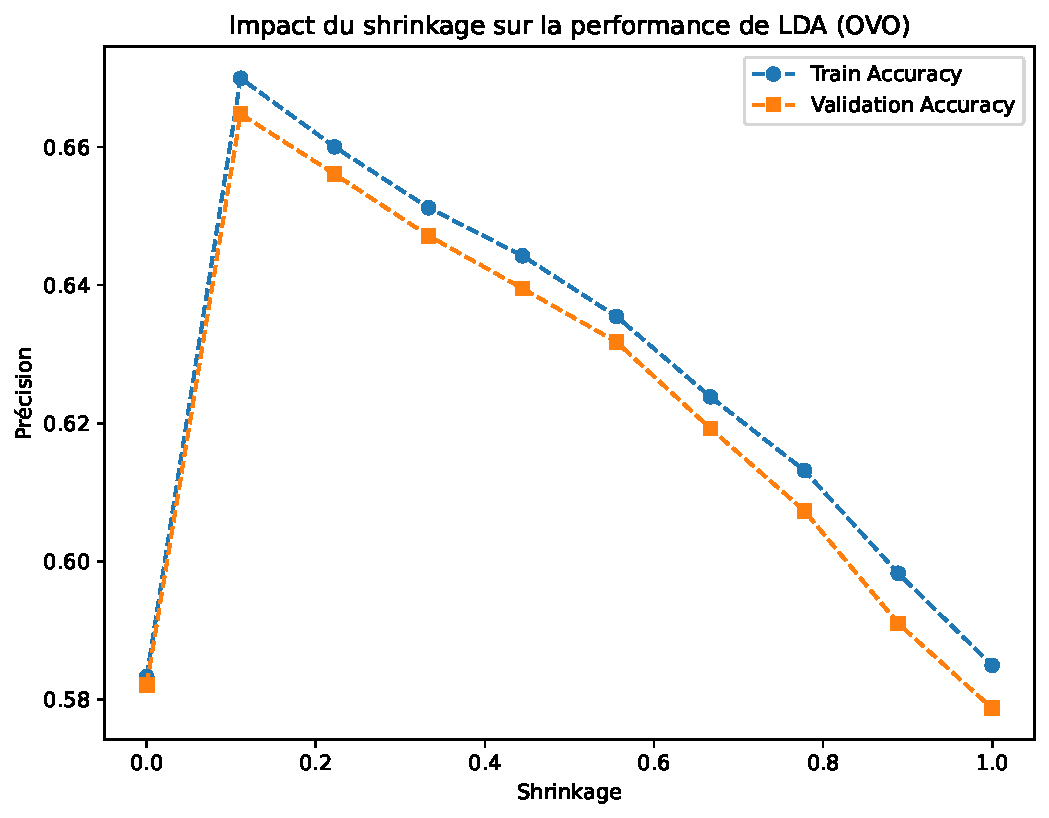
\includegraphics[keepaspectratio]{lda_ovo_files/figure-pdf/cell-2-output-2.pdf}}

\begin{verbatim}

Matrice de confusion (OVO) :
[[1198  687    1    0    7    2  224]
 [ 448 2160   82    1   59   70   13]
 [   0   66 1197   75    5   87    0]
 [   0    0   48   50    0   12    0]
 [   7  205   26    0  124   18    0]
 [   0   82  366    4    2  240    0]
 [ 139   13    3    0    2    0  664]]

Évaluation sur l'ensemble de test
              precision    recall  f1-score   support

           1       0.67      0.57      0.61      2119
           2       0.67      0.76      0.71      2833
           3       0.69      0.84      0.76      1430
           4       0.38      0.45      0.42       110
           5       0.62      0.33      0.43       380
           6       0.56      0.35      0.43       694
           7       0.74      0.81      0.77       821

    accuracy                           0.67      8387
   macro avg       0.62      0.59      0.59      8387
weighted avg       0.67      0.67      0.66      8387
\end{verbatim}




\end{document}
